\documentclass[12pt,a4paper,twopage]{article}
\usepackage[utf8]{inputenc}
\usepackage{geometry}
\geometry{a4paper,left=30mm,right=30mm, top=3cm, bottom=30mm} 
\usepackage{multicol}
\usepackage{amsmath}
\usepackage{float}
\usepackage{epsfig,graphicx}
\usepackage{xcolor,import}
\usepackage{subcaption}
\usepackage[font=small,labelfont=bf]{caption}
\usepackage{siunitx}
\usepackage[german]{babel}
\usepackage{textcomp}
\usepackage{mathtools}
\linespread{1.1}
\usepackage{parskip}
\setlength{\parindent}{12pt}


\begin{document}


\thispagestyle{empty}
			\begin{center}
			\Large{Fakultät für Physik}\\
			\end{center}
\begin{verbatim}


\end{verbatim}
							%Eintrag des Wintersemesters
			\begin{center}
			\textbf{\LARGE SOMMERSEMESTER 2015}
			\end{center}
\begin{verbatim}


\end{verbatim}
			\begin{center}
			\textbf{\LARGE{Physikalisches Praktikum II}}
			\end{center}
\begin{verbatim}




\end{verbatim}

			\begin{center}
			\textbf{\LARGE{PROTOKOLL}}
			\end{center}
			
\begin{verbatim}





\end{verbatim}

			\begin{flushleft}
			\textbf{\Large{Experiment (Nr., Titel):}}\\
			PS9, Heißluftmotor - Stirlingprozess
							%Experiment Nr. und Titel statt den Punkten eintragen
			\LARGE{}	
			\end{flushleft}

\begin{verbatim}

\end{verbatim}	
							%Eintragen des Abgabedatums, oder des Erstelldatums des Protokolls
			\begin{flushleft}
			\textbf{\Large{Datum:}} \Large{29.5.2015}
			\end{flushleft}
			
\begin{verbatim}
\end{verbatim}
							%Namen der Protokollschreiber
		\begin{flushleft}
			\textbf{\Large{Bachleitner Veronika, Grafendorfer Erik}} 
			\end{flushleft}

\begin{verbatim}


\end{verbatim}
							%Kurstag und Gruppennummer, zb. Fr/5
			\begin{flushleft}
			\textbf{\Large{Kurstag/Gruppe:}} \Large{FR/1}
			\end{flushleft}

\begin{verbatim}






\end{verbatim}
							%Name des Betreuers, das Praktikum betreute.
			\begin{flushleft}
			\LARGE{\textbf{Betreuer:\Large{ }}}		
			\end{flushleft}
			
\section{Aufgabenstellung}

\section{Theorie}
\subsection{Allgemeine Grundlagen}
Es gibt thermodynamische Kreisprozesse, bei denen durch verschiedene Zustandsänderungen einem System Wärme zugeführt oder entnommen wird. Solche Zustandsänderungen sind isotherm (Temperatur konstant), adiabatisch (Wärmemenge konstant) und isochor (Volumen konstant).
\subsubsection{Carnot Prozess}
Eine Carnot-Maschine benützt eine Arbeitssubstanz, mit der sie einen quasistatischen Kreisprozess ausführt:\\
\\
1. Isotherme Zustandsänderung (Expansion). Dabei nimmt as Arbeitsgas die Wärmemenge $Q_{zu}$ auf.\\
2. Adiabatische Zustandsänderung (Expansion). Dabei hat das Arbeitsgas am Ende die Temperatur $T_2$.\\
3. Isothemre Zustandsänderung (Kompression). Dabei gibt as Arbeitsgas die Wärmemenge $Q_{ab}$ ab.\\
4. Adiabatische Zustandsänderung (Kompression). Dabei hat das Arbeitsgas am Ende die Temperatur $T_1$.\\
\\
Technisch ist der Carnot-Prozess jedoch nicht durchführbar, da einerseits die direkte Abfolge dieser Zustandsänderungen nicht realisierbar und andererseits die Prozesse in den meisten Wärmekraftmaschinen nicht reversibel sind.\\
\\
Der Wirkungsgrad ist gegeben durch:
$$\eta=\frac{A}{Q_{zu}}=\frac{Q_{zu}-Q_{ab}}{Q_{zu}}=1-\frac{Q_{ab}}{Q_{zu}}$$
wo $A$ die Arbeit und $Q_{zu}$ bzw. $Q_{ab}$ die zugeführte bzw. abgeführte Wärmemenge sind.\\
\\
Der Stirling-Kreisprozess besteht aus isothermen und isochoren Zustandsänderungen:\\
\\
1. Isotherme Zustandsänderung (Expansion).\\
2. Isochore Zustandsänderung (Expansion).\\
3. Isotherme Zustandsänderung (Kompression).\\
4. Isochore Zustandsänderung (Kompression).\\
\\
Verwendet man die ideale Gasgleichung ($pV=NkT$) sowie die Formeln für die Zustandsänderungen erhält man für den (idealen) Wirkungsgrad:
$$\eta=\frac{T_1-T_2}{T_1}=1-\frac{T_2}{T_1}$$
Der reale Wirkungsgrad ist dann gegeben durch
$$\eta_{real}=\frac{P_{Motor}}{P_{zu}}$$
wo $P$ die Leistung (Motor bzw. zugeführt) ist. Die Leistung kann in unserem ersten Versuch auch über folgendes Skalarprodukt bestimmt werden:
$$P=\vec{M}\cdot\vec{\omega}=\vec{F}\times\vec{r}\cdot\vec{\omega}$$
wo $\vec{M}$ das Bremsdrehmoment, $vec{F}$ die Kraft, $\vec{r}$ der Radius und $\vec{\omega}$ die Winkelgeschwindigkeit ist.\\
\\
Bei der \textit{Stirling-Maschine als Kältemaschine} wird im Prinzip ein Kreisprozess wie der oben beschrieben durchgeführt. Da es sich allerdings um eine Kältemaschine handeln soll, wird der Kreispozess jedoch gegen den Uhrzeigersinn durchlaufen.

\section{Aufbau}
\subsection{Wärmekraftmaschine}
\subsection{Kältemaschine}

\section{Durchführung}

\subsection{Wärmekraftmaschine}
\subsection{Kältemaschine}

\section{Ergebnisse}
\subsection{Wärmekraftmaschine}

\begin{center}
\begin{figure}[H]
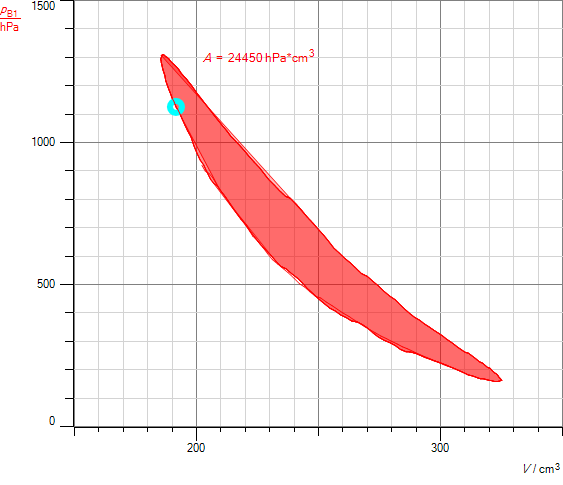
\includegraphics[scale=0.7]{bachgraf/heissluft.png}
\caption{P-V-Diagramm der Wärmekraftmaschine mit angegebener Arbeit (Flächeninhalt).}
\label{fig:heissluft-pv}
\end{figure}
\end{center}

In Abbildung \ref{fig:heissluft-pv} ist das P-V-Diagramm der Wärmekraftmaschine zu sehen. Die Fläche unter der Kurve, und damit die Arbeit, wird vom Programm berechnet als:
$$A=24450hPa cm^3 =(2.445 \pm 0.001) Ws$$
\\
Mit dem Stroboskop kann die Leerlauf-Frequenz gemessen werden:
$$f_0=(5.26 \pm 0.01)Hz$$
\\
Wenn wir die mechanische Arbeit mit der Leerlauf-Frequenz $f_0$ multiplizieren erhalten wir die ideale Leistung des Motors:
$$\boxed{P_{ideal}=(12.861 \pm 0.025)W}$$
\\
Die zugeführte Leistung ergibt sich aus folgenden Strom- bzw. Spannungswerten: 
$U=(11 \pm 1)V$, $I=(13 \pm 1)A$
$$\boxed{P_{zu}=U \cdot I = (143 \pm 17)W}$$
Die Unsicherheit der zugeführten Leistung ergibt sich aus:
$\sqrt{(U\cdot\Delta I)^2+(I\cdot\Delta U)^2}=\sqrt{11^2+13^2}\approx17.029$
\\
Aus der idealen und der zugeführten Leistung können wir den idealen Wirkungsgrad berechnen:
$$\boxed{\eta_{ideal}=\frac{P_{ideal}}{P_{zu}}=(9.0 \pm 0.1)\%}$$
\\
Als nächstes wird der reale Wirkungsgrad des Motors bestimmt, indem wir mit dem Prony'schen Bremszaum eine Leistung unter Belastung abnehmen.
Wir stellen anhand der Federwaage folgende Bremskraft fest:
$$F=(0.62-0.16 \pm 0.01)N=(0.46 \pm 0.01)N$$
wobei die abgezogenen $0.16$ den Nullpunkt auf der Federwaage markieren.\\
\\
Die Frequenz war dabei
$$f=(4.29 \pm 0.01)Hz$$
\\
Den Radius des Bremszaums haben wir nicht selbst gemessen aber bei Mitstudenten erfragt: $r=(0.250 \pm 0.002)m$\\
\\
Aus diesen drei Werten können wir uns den realen Wirkungsgrad berechnen.\\
Das Bremsdrehmoment ist $\vec{M}=\vec{F}\times \vec{r}=F\cdot r = (0.115 \pm 0.003)Nm$ und die reale Leistung is daraus:
$$\boxed{P_{real}=M\cdot f=(0.49 \pm 0.01)Ws}$$
\\
Daraus erhalten wir schließlich den realen Wirkungsgrad:
$$\boxed{\eta_{real}=\frac{P_{real}}{P_{zu}}=(0.35 \pm 0.05)\%}$$
\subsection{Kältemaschine}

\begin{center}
\begin{figure}[H]
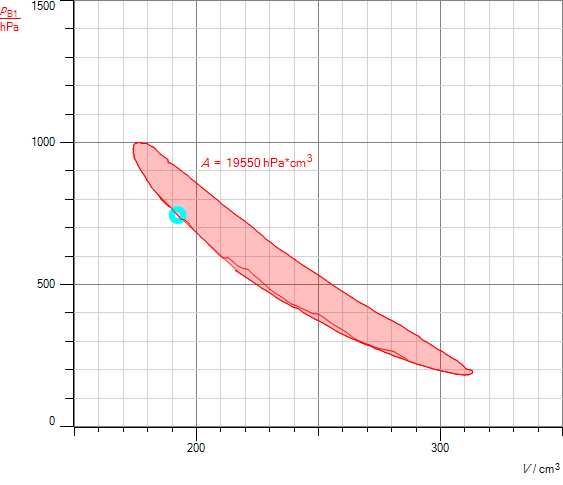
\includegraphics[scale=0.7]{bachgraf/kaeltemaschine.png}
\label{kaeltemaschine-pv}
\end{figure}
\end{center}

Erste Messung:
$8.2^\circ C$ bei $(350 \pm 10)mA$ und $(240 \pm 10)V$, Heizleistung: $(7.0 \pm 0.5)V$ $(1.5 \pm 0.1)A$\\


$8.0^\circ C$ bei $(350 \pm 10)mA$ und $(240 \pm 10)V$, Heizleistung: $(8.0 \pm 0.5)V$ $(1.7 \pm 0.1)A$, Frequenz: $f=4.63Hz$\\


\section{Diskussion}
\subsection{Wärmekraftmaschine}
\subsection{Kältemaschine}
Werte für andere Temperaturen haben wir nicht aufgeschrieben: Die Unsicherheiten der Strom- und Spannungsmessungen sind so groß bzw. genauer gesagt der Zeiger auf den analogen Messgeräten schwankt so sehr, dass die Werte für Strom und Spannung sich bei unterschiedlichen Temperaturen nicht sichtbar unterscheiden.
																						
\end{document}
